\subsection*{Problema 19}

\textbf{Enunciado:} Calcular la integral:\\
$\displaystyle \int \dfrac{(1 - \sin x)\cos x \, dx}{\sin x + \sin^2 x}$

\textbf{Solución:}

Para resolver la integral dada, utilizaremos el método de sustitución algebraica. Observamos que la derivada de $\sin x$ es $\cos x \, dx$, lo cual sugiere el cambio de variable:

\begin{align*}
u &= \sin x \\
du &= \cos x \, dx
\end{align*}

Sustituyendo estas expresiones en la integral original, obtenemos una función racional en términos de $u$:

\begin{align*}
I &= \int \dfrac{(1 - u) \, du}{u + u^2} \\
I &= \int \dfrac{1 - u}{u(1 + u)} \, du
\end{align*}

Ahora, descomponemos el integrando en fracciones parciales de la forma general:

\begin{align*}
\dfrac{1 - u}{u(1 + u)} &= \dfrac{A}{u} + \dfrac{B}{1 + u}
\end{align*}

Multiplicando ambos lados por el denominador común $u(1 + u)$:

\begin{align*}
1 - u &= A(1 + u) + Bu
\end{align*}

Para hallar las constantes $A$ y $B$, evaluamos en valores convenientes de $u$:

\begin{align*}
\text{Si } u = 0 &\implies 1 = A(1) \implies A = 1 \\
\text{Si } u = -1 &\implies 1 - (-1) = B(-1) \implies B = -2
\end{align*}

Sustituyendo los valores de $A$ y $B$ en la integral, se tiene:

\begin{align*}
I &= \int \left( \dfrac{1}{u} - \dfrac{2}{1 + u} \right) du
\end{align*}

Integramos cada término por separado:

\begin{align*}
I &= \ln|u| - 2\ln|1 + u| + C
\end{align*}

Aplicando las propiedades de los logaritmos:

\begin{align*}
I &= \ln|u| - \ln((1 + u)^2) + C \\
I &= \ln\left| \dfrac{u}{(1 + u)^2} \right| + C
\end{align*}

Finalmente, regresamos a la variable original $x$ sustituyendo $u = \sin x$:

\begin{align*}
I &= \ln\left| \dfrac{\sin x}{(1 + \sin x)^2} \right| + C
\end{align*}

\begin{figure}[H]
	\centering
	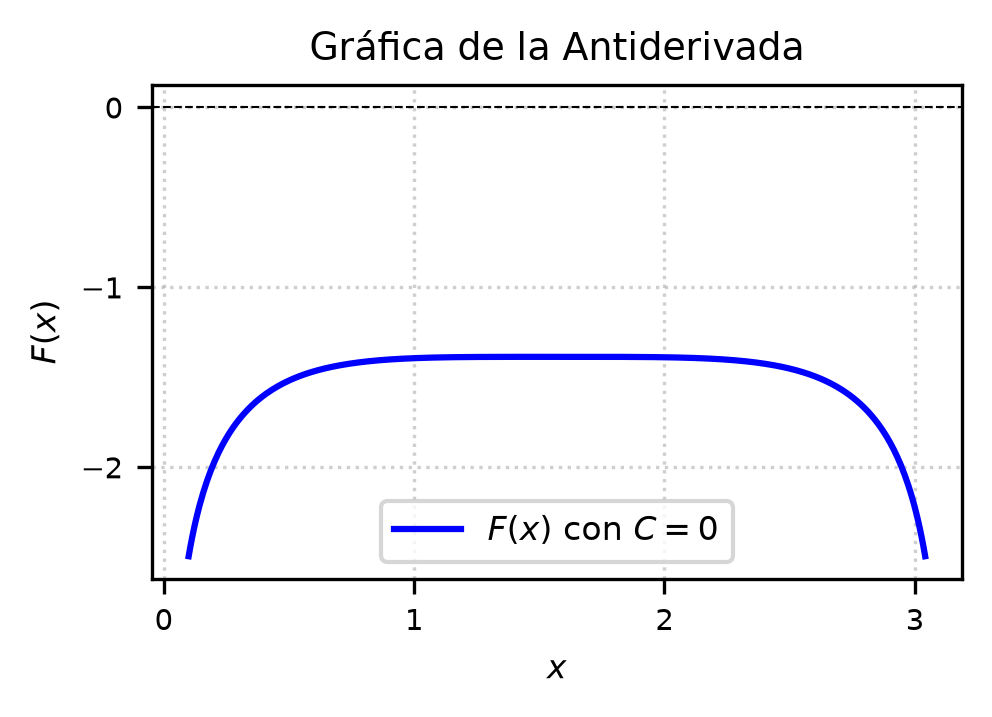
\includegraphics[width=\columnwidth]{semana_04/graficas/SEM04_P19_grafica.png}
	\caption{Representación gráfica de $f(x)$ y su antiderivada $F(x)$ evaluada para la constante de integración $C = 0$ (Problema 19).}
	\label{fig:problema19}
\end{figure}
